\chapter{IF stage}
\label{chap:if}

In this chapter we will show how the IF stage is structured and how each block works.
In figure \ref{fig:IF_stage} the block diagram of the stage is shown.

\begin{figure}[!ht]
	\centering
	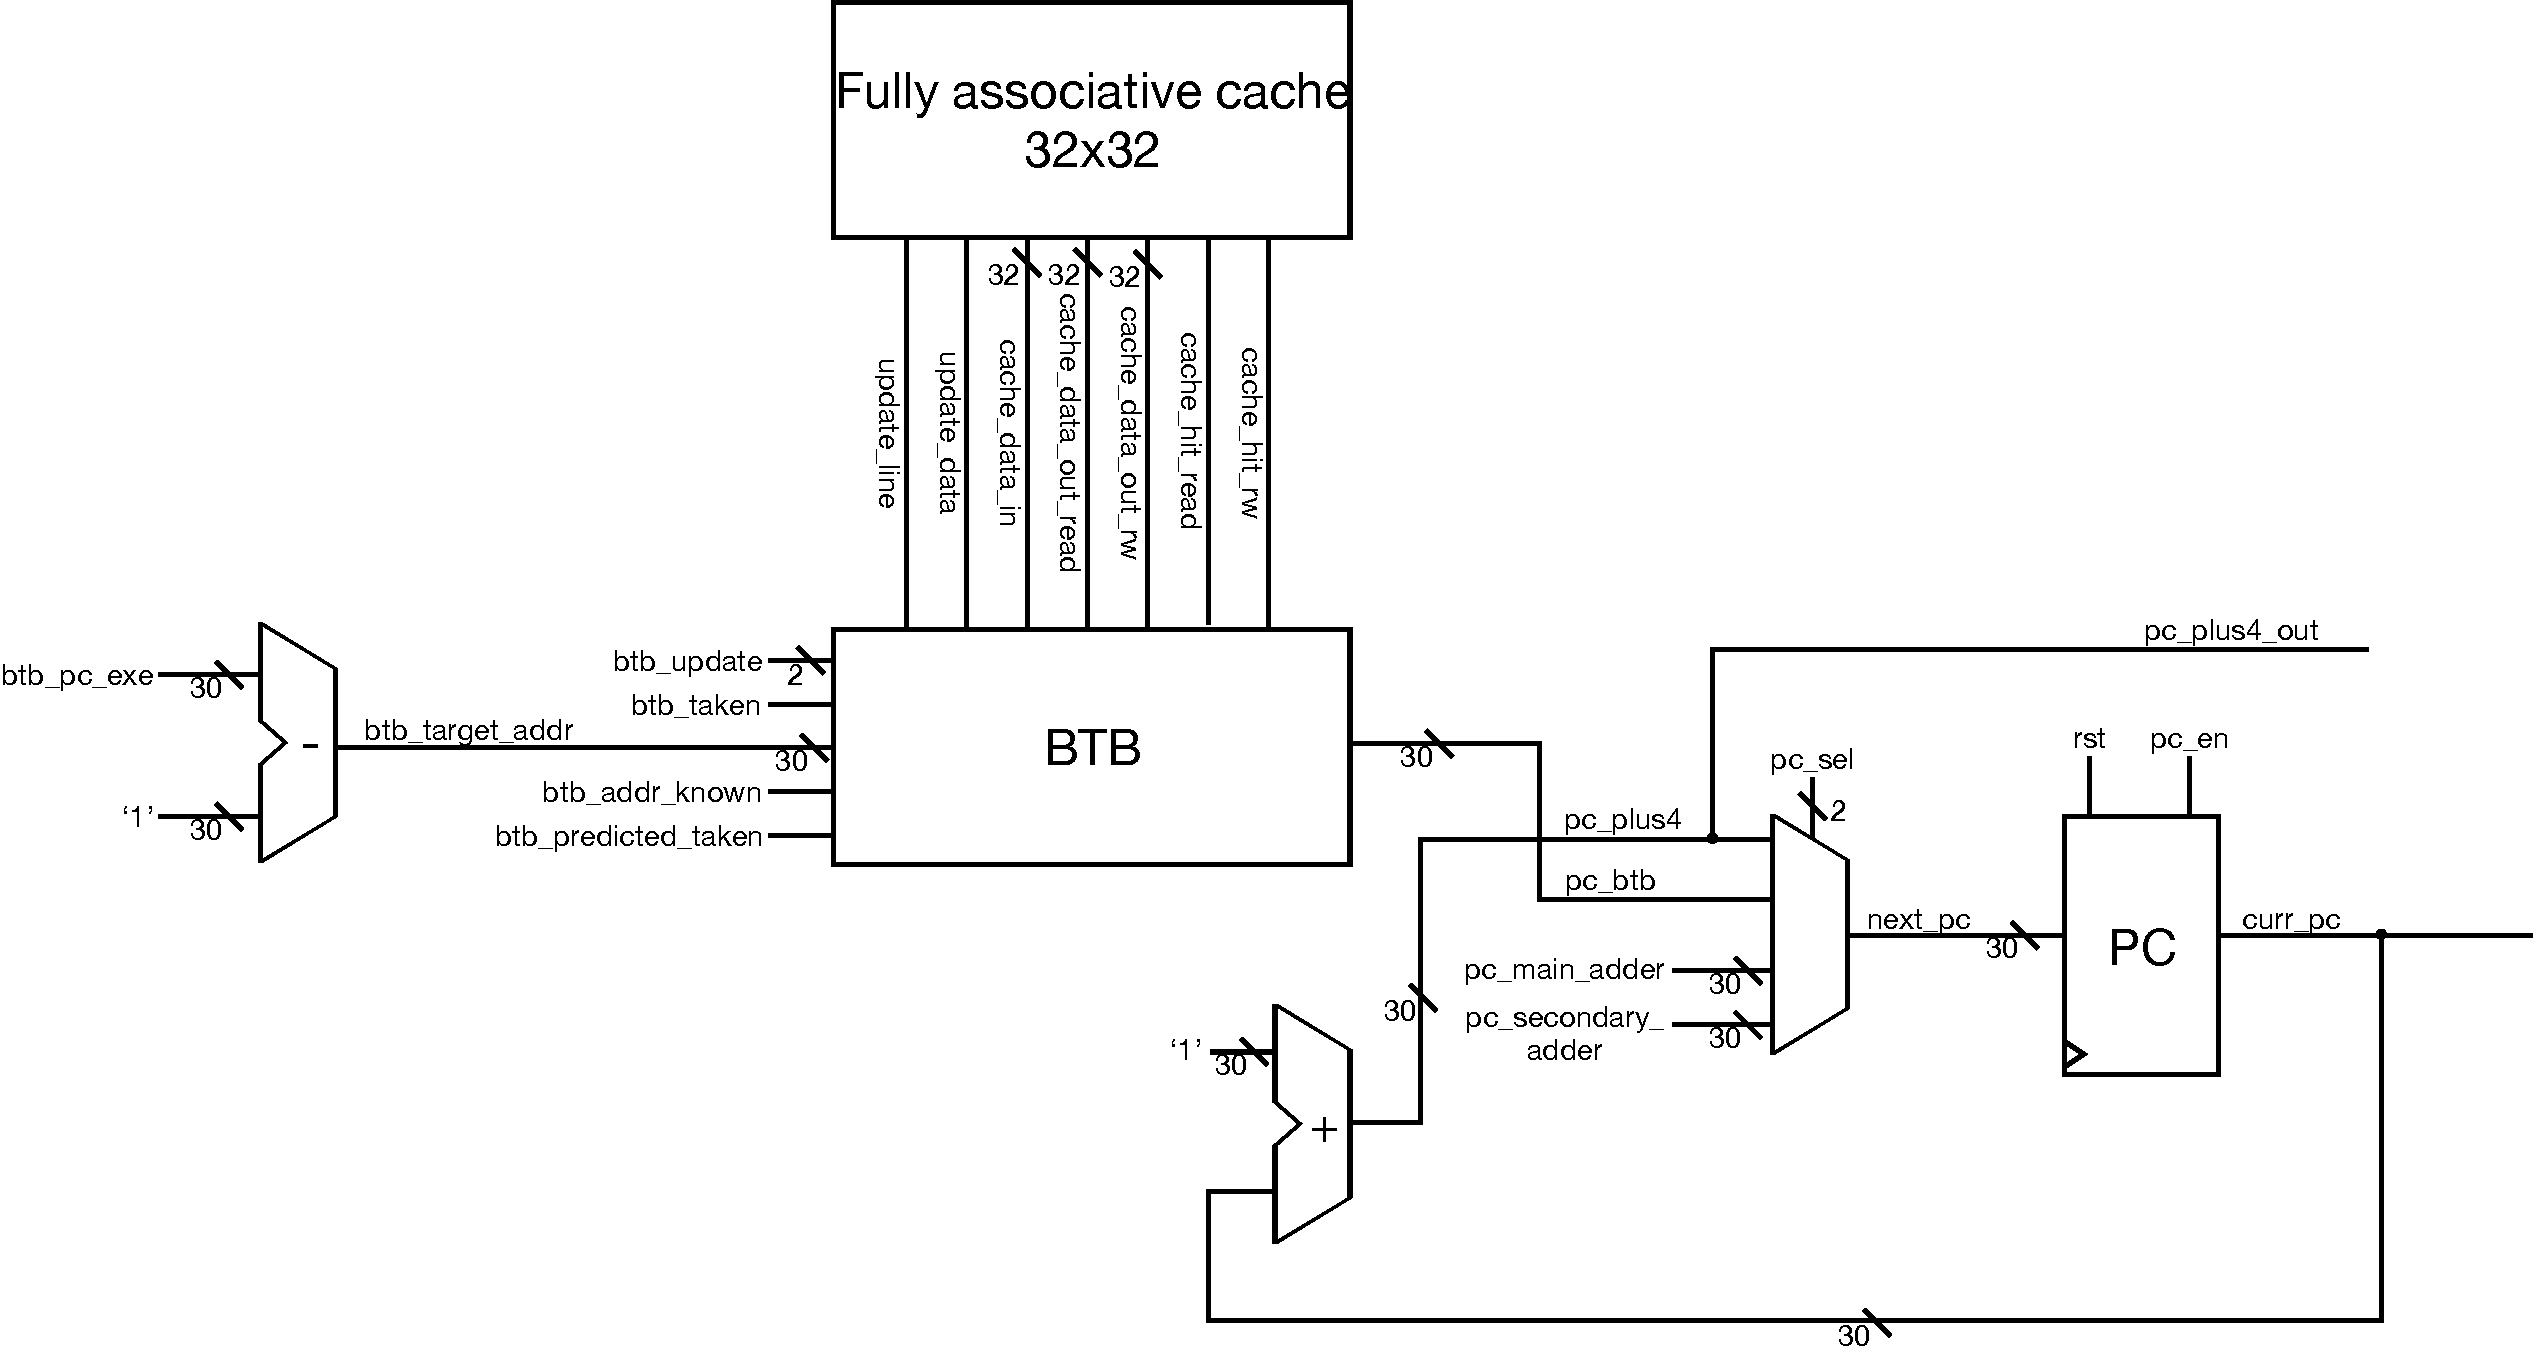
\includegraphics[width=\linewidth]{./chapters/figures/IF_stage.pdf}
	\caption{Block diagram of the IF stage}
	\label{fig:IF_stage}
\end{figure}

There are:

\begin{enumerate}
    \item a register storing the value of the current PC.
    \item A mux that selects among its 4 inputs which will be the next PC value.
    \item An adder that calculates $current\ pc + 4$
    \item A {\it Branch Target Buffer} (BTB) able to recognize and predict the behavior of known branches and jumps
    \item A 32-entries, 32 bits, fully associative cache that it is used by the BTB to recognize known branches and jumps
    \item A subtractor calculating $btb\ pc\ exe - 4$, that is the PC of the instruction in the EXE stage. It is used when updating the BTB content.
\end{enumerate}

In this stage the PC is used on 30 bits instead of 32 because instructions are aligned on 32 bits boundaries, therefore the 2 LSBs are always 0
and it was useless to add more HW to handle them.

\section{Branch Target Buffer}

The {\it branch target buffer} is a hardware structure used to known in the IF stage if the instruction being fetched is a known branch or jump.
It does so by accessing in read mode its cache using as address the current pc (this connection is not shown in figure \ref{fig:IF_stage}). For the differences
between read mode and write mode of the cache refer to subsection \ref{subsec:fully_cache}.
Our BTB operates over 3 values, as shown in figure \ref{fig:BTB_fields}.

\begin{figure}[!ht]
    \centering
    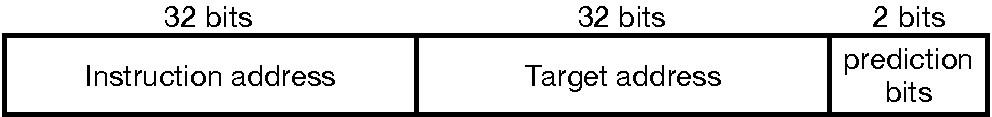
\includegraphics[width=\linewidth]{./chapters/figures/BTB_fields.pdf}
	\caption{Branch target buffer values}
	\label{fig:BTB_fields}
\end{figure}

\begin{enumerate}
    \item The {\it instruction address} is the memory address where the instruction resides. In our implementation corresponds to the TAG value in the cache.
    \item The {\it target address} is where the PC branch or the jump would go in case the jump condition is verified.
    \item The {\it prediction bits} are used by the FSM inside the BTB to predict whether a branch will be taken or not. The state machine of the prediction bits is shown in figure \ref{fig:BTB_FSM}.
\end{enumerate}

The target address, concatenated with the prediction bits, form a 32 bit value which corresponds to the data stored inside the cache.\\
Now let's take a closer look to the FSM implementation.

\begin{figure}[!ht]
	\centering
	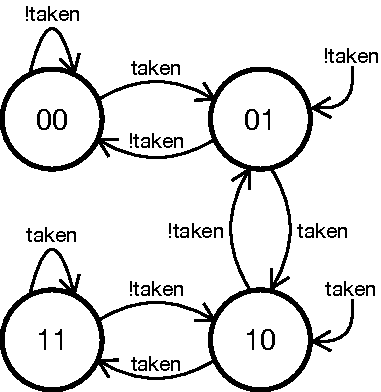
\includegraphics[width=0.3\linewidth]{./chapters/figures/BTB_FSM.pdf}
    \caption{Branch target buffer FSM representation}
    \label{fig:BTB_FSM}
\end{figure}

There are two entry points in the FSM: one that enters the state \verb|01| and one that enters the state \verb|10|. The former is used to add a new branch as non-taken,
while the latter is used for the opposite. In the delivered implementation only the {\it taken} entry point is used, but since at the beginning of the development we did not
know if we would have added also non-taken branch to the BTB, we felt that this degree of flexibility would have been nice to have.

Besides this particular, the FSM is straightforward: the 2 bits are used to store the state of a branch, and their values have the following meanings:

\begin{enumerate}
    \item \verb|00|: strongly not taken.
    \item \verb|01|: weakly not taken.
    \item \verb|10|: weakly taken.
    \item \verb|11|: strongly taken.
\end{enumerate}

The value of \verb|btb_taken| is 0 for the first two cases and 1 for the last two, provided that the address that is being considered is known to the cache (that is, we have $hit = 1$ in read mode).

The BTB of course needs to be updated every time a branch is executed or discovered. This is achieved by writing in \verb|btb_update| \verb|01| to update only the history bits or \verb|10| to add a new
branch, by concatenating the target address to the history bits and by setting the cache's write address to the instruction's PC.

\subsection{Fully associative cache}
\label{subsec:fully_cache}

A key component of the BTB is the cache, where as already said all the known branches and jumps are stored. We decided to use a 32-entries fully associative cache to have the highest possible hit rate,
since every miss could hurt the pipeline's performance. Its general, simplified structure is shown in figure \ref{fig:BTB_cache}.

\begin{figure}[!ht]
	\centering
	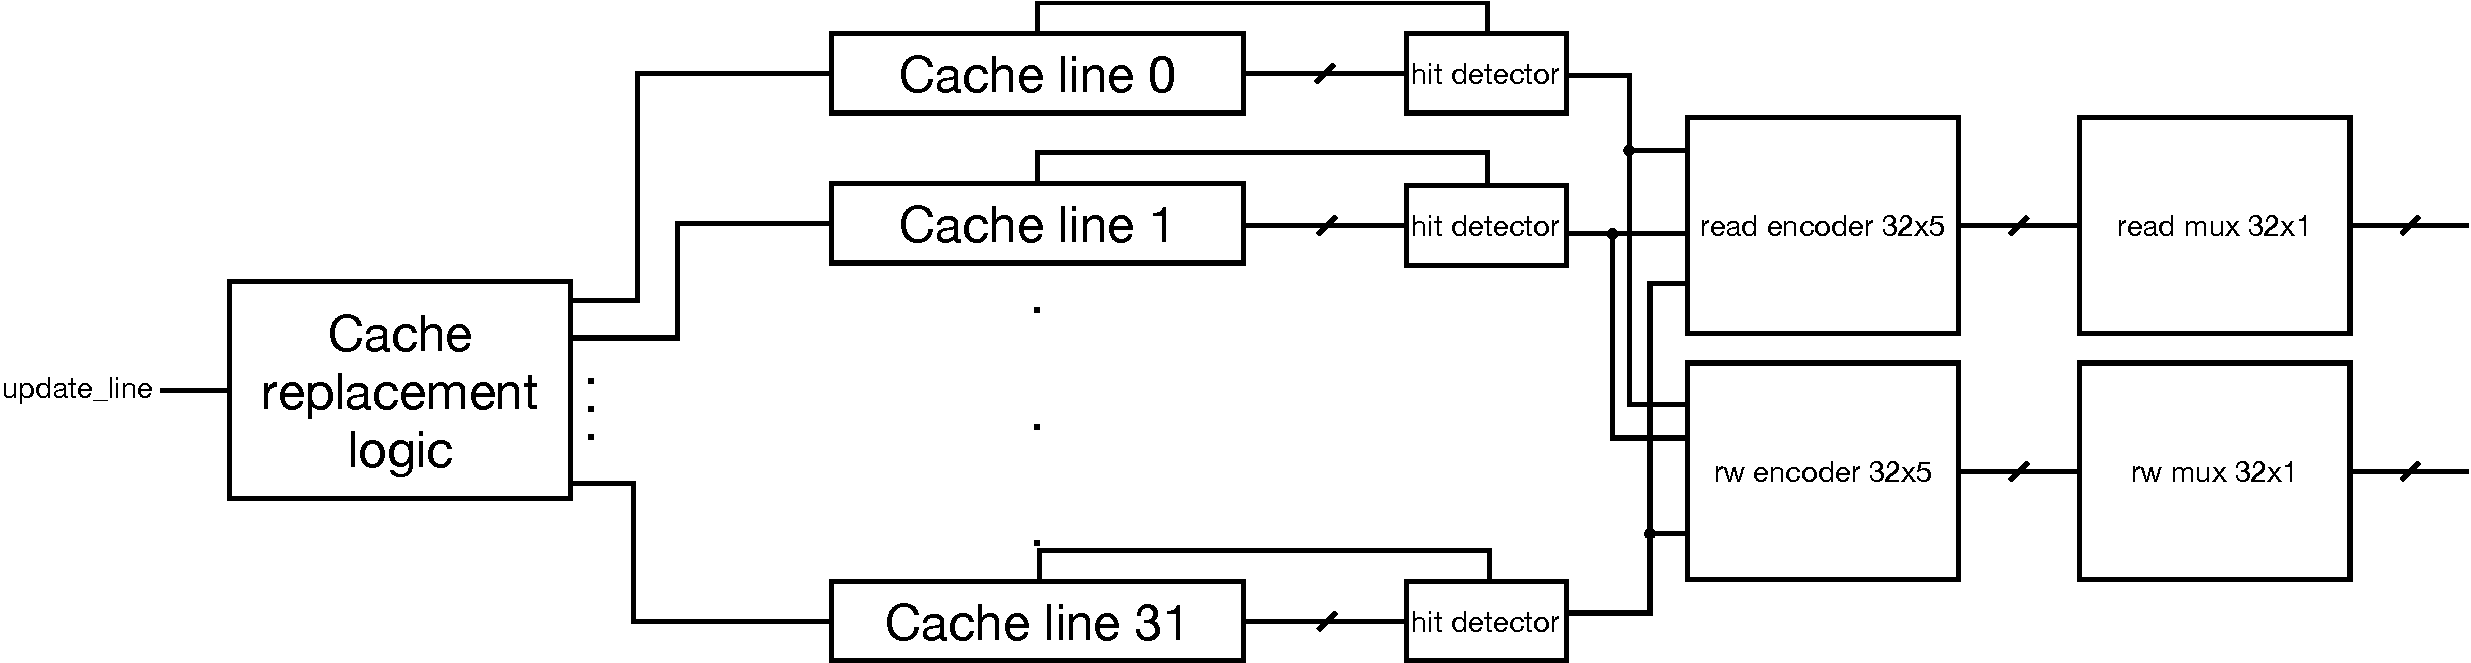
\includegraphics[width=\linewidth]{./chapters/figures/BTB_cache.pdf}
    \caption{Cache general representation}
    \label{fig:BTB_cache}
\end{figure}

This cache support two read operations and a write operation per clock cycle and implements a FIFO replacement logic. Each cache line has a hit detector, which is used to detects a hit in case of a read, and
to issue a line update (only the data is updated, not the tag) if requested by the BTB. The hits signals then enter two 32-entries encoders which in turn drive two 32-entries muxes, used to output the data from the cache.
To illustrate exactly how a cache line and a hit detector work we'll refer to picture \ref{fig:BTB_cache_line}.

\begin{figure}[!ht]
	\centering
	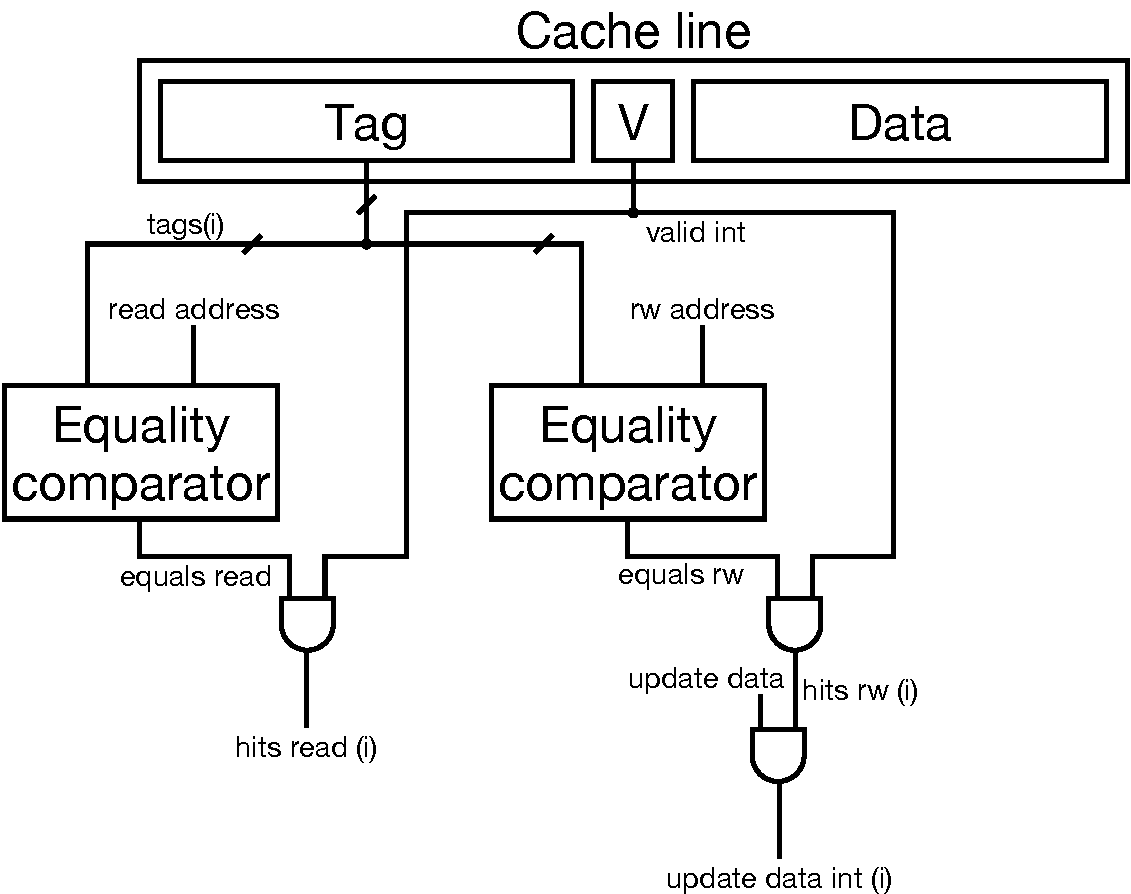
\includegraphics[width=0.6\linewidth]{./chapters/figures/BTB_cache_line.pdf}
    \caption{Cache line and hit detectors}
    \label{fig:BTB_cache_line}
\end{figure}

A cache line is composed of a 30 bits \verb|tag| field, that stores the PC of the branch/jump, a validity bit used to discriminate invalid data after a reset and a 32 bits \verb|data| field that keeps the value
of the target address along with the history bits. The tag enter two equality comparators to check if a match exists either with the read address, the write address, or both. To determine if a hit has occurred this
is not sufficient though, because the data stored in the tag may be invalid. To solve this issue an AND is executed between the validity bit and each comparator's output. The write part has an additional AND between
its hit value and the \verb|update_data| signal to determine if this line have to update its \verb|data| field.

\section{Program counter selection}

There are 4 possible next program counter values to choose at each clock cycle:
\begin{enumerate}
    \item $PC + 4$
    \item $PC_{BTB}$
    \item $PC_{main\ adder}$
    \item $PC_{secondary\ adder}$
\end{enumerate}

$PC + 4$ is the default choice when the BTB doesn't recognize the address and the EXE have not executed a branch or a jump. $PC_{BTB}$ is taken whenever the BTB recognizes the address and the EXE have not executed
any branch or jump. $PC_{main\ adder}$ is used when the EXE have executed a \verb|jr| or \verb|jalr|. Finally, $PC_{secondary\ adder}$ is the value used when any branch or jump except \verb|jr| and \verb|jalr| is
executed in the EXE stage.